\section{Technical}\label{sec:technical}

\subsection{Inference Rules}
Previous work takes advantage of model-checking approach to check whether a
specific C/C++11 trace is sequentially consistent. By building up edges
(\textit{sb}, \textit{rf} and \textit{sc} by implication rules) between atomic
operations, it judges whether the trace is SC by whether there exists a cycle in
that graph. Besides, when it finds a non-SC trace, it has a sorting algorithm
that generates an SC-like trace and exposes which reads-from edge that causes a
cycle.

Under the C/C++11 memory model, inferring the ordering parameters to obtain SC
behaviors is essentially a searching problem. In the absence of consume
operations, memory order parameters for atomic operations can be only one of the
following: \textit{memory\_order\_relaxed}, \textit{memory\_order\_release},
\textit{memory\_order\_acquire}, \textit{memory\_order\_acq\_rel} and
\textit{memory\_order\_seq\_cst}. By enumerating all possible memory order
parameters, we can guarantee that we can find out all the possible inference of
parameters that ensure SC behaviors for a specific test case. However, this
naive approach obviously leads to an exponential searching space.

Actually, when we have a non-SC execution, we have some knowledge availabe
reflecting where the problem may lie. Consider we start from the case where all
memory order parameters are \textit{memory\_order\_relaxed}. Whenever the
model-checking approach finds out a cycle in a specific execution, we have to
infer some stronger memory orders to eliminate the cycle. What causes the cycle
to happen leads to the non-SC trace. We propose a search-based approach combined
with cycle patterns and their fixes to reduce searching space.

Among those non-SC executions, previous work will reorder the original trace to
yield an SC-like trace which indicates where a bad read-from edge happens.  In
Figure~\ref{fig:fence_implications} , we show the two universal patterns
that can exist in cycles. We explain how we should fix the cycle patterns
respectivelys the following.


\mypara{\bf Old value read:} \textit{Patter a} in
Figure~\ref{fig:fence_implications} shows the case where a load reads
its value from an old store rather than the recent store. \textit{isc} is
the union of \textit{sc}, \textit{hb}, \textit{rf} and the implied edges. If any one of
the two \textit{isc} edge is not \textit{hb}, we will impose either \textit{hb} or
\textit{sc} to it. If an \textit{isc} edge is the union of \textit{rf},
\textit{hb}, we can use release/acquire pair to establish synchronization;
otherwise, we will make both operation sequentially consistent. For the latter
case, it can be insufficient to get rid of the execution. However, by
proritizing the \textit{sc} edges in building the graph, a different problematic
spot will be found, and we can fix the cycles iteratively. Also, when both
\textit{isc} edges are implied edges, we need to explore the cases where there
exist other loads that are \textit{isc-ordered} after the old store and before
the read.


\mypara{\bf Future value read:} \textit{Pattern b} in
Figure~\ref{fig:fence_implications} shows a load that is \textit{isc-ordered}
before a store reads its value from that store (or reading the future value).
The two possbile fixes is: 1) impose \textit{hb} between the store and the load,
which can be easily done by using release/acquire; 2)impose \textit{hb} or
\textit{sc} between the load and the store, which is similar to what we
discussed in \textit{pattern a}.

Figure~\ref{fig:algorithm} shows the core searching algorithm for all possible
parameters.

\begin{figure}[!ht]
\centering
\begin{tabular}{cc}
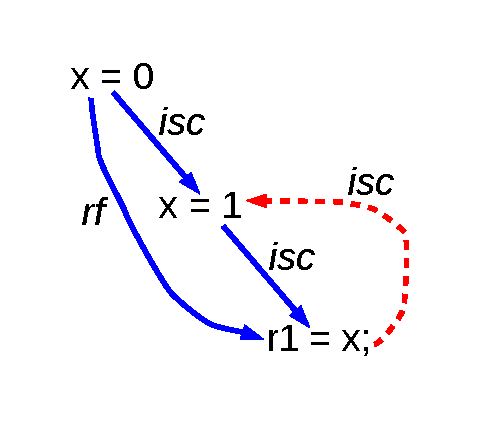
\includegraphics[scale=.45]{figures/old_val_isc}&
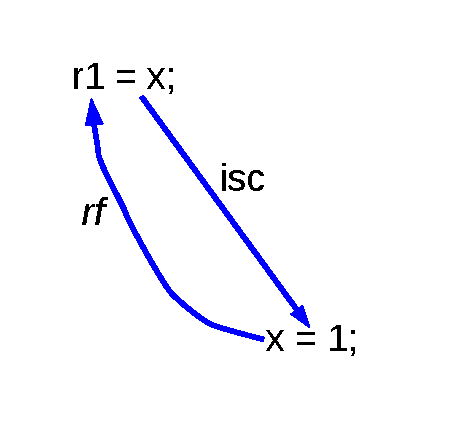
\includegraphics[scale=.45]{figures/future_val_isc}\\
Old Value Read&Future Value Read\\
\textit{(pattern a)}&\textit{(pattern b)}
\end{tabular}
\caption{\label{fig:fence_implications}Cycle Patterns for Non-SC Behaviors}
\end{figure}


\begin{figure}[!ht]
\centering
\begin{tabular}{c}
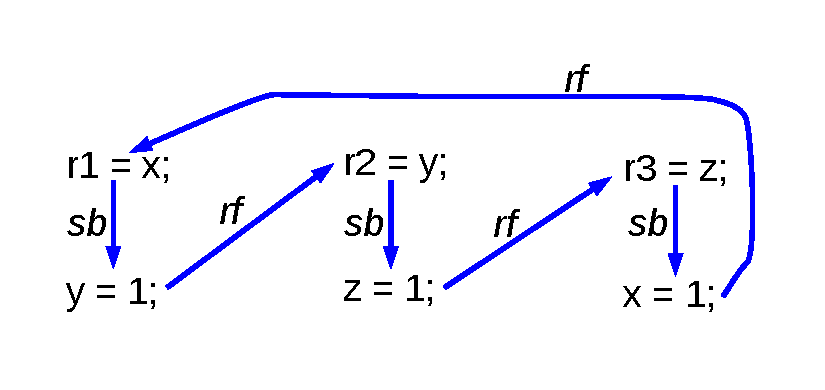
\includegraphics[scale=.45]{figures/examples/circular_rf}\\
Circular Reads-from\\
\hline\\
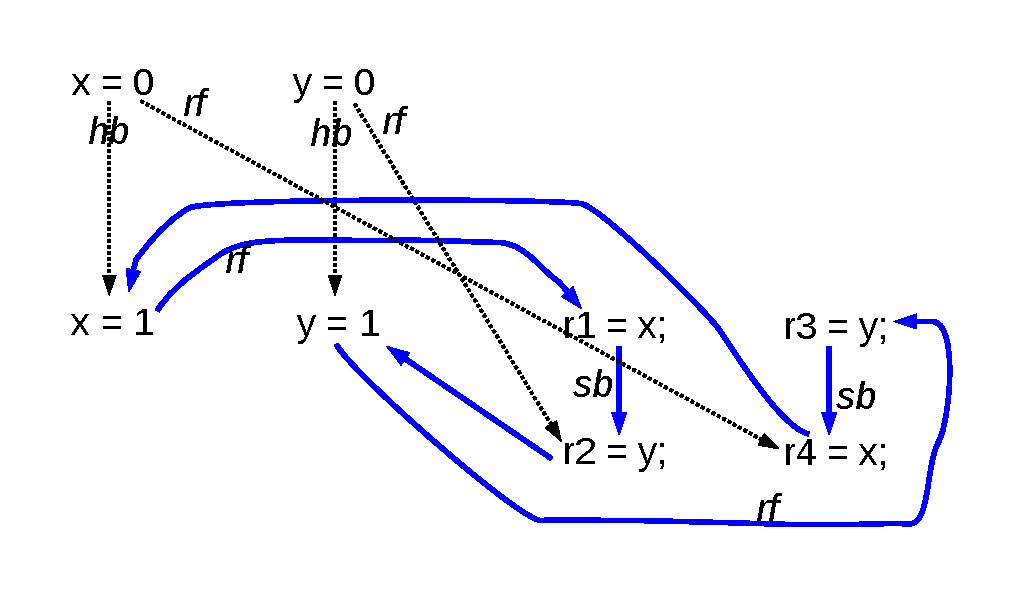
\includegraphics[scale=.45]{figures/examples/iriw}\\
Independent Reads \& Independent Writes\\
\hline\\
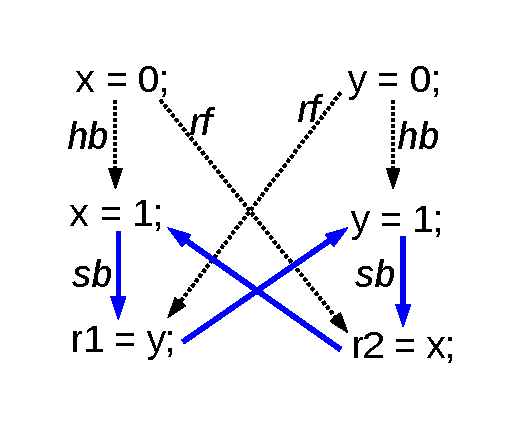
\includegraphics[scale=.45]{figures/examples/peterson_lock}\\
Peterson Lock\\
\hline\\
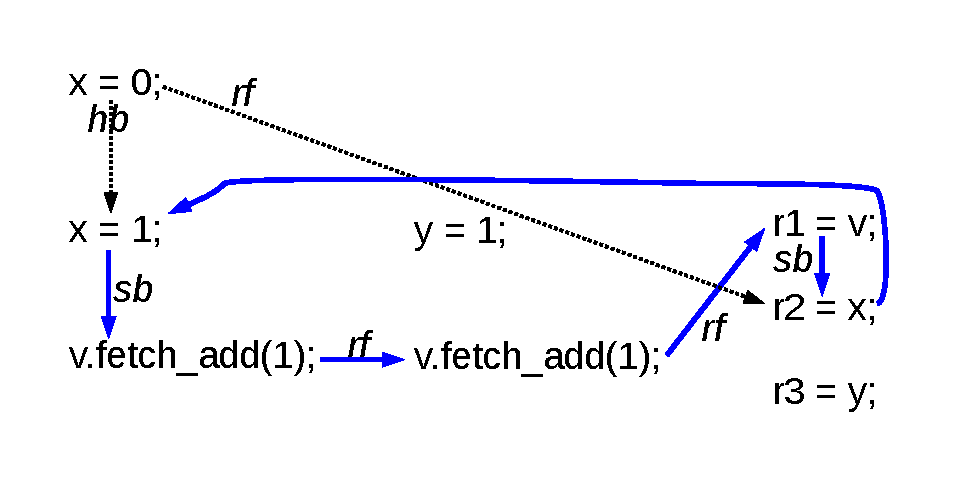
\includegraphics[scale=.45]{figures/examples/release_seq}\\
Release Sequence\\
\end{tabular}
\caption{\label{fig:nonsc_example}Non-SC Examples}
\end{figure}

\begin{figure}[!htbp]
\begin{algorithmic}[1]
\Function{InferParams}{}
\State candidates := \{\}
\State candidate $c1$ := replace all wildcards with \textit{relaxed}
\State candidates += $c1$
\State results := \{\}
\While{candidates is not empty}
\State Candidate $c$ := candidates.pop()
\State Model-check with $c$ and yield a cycle $l$
\If{$l$ == NULL}
\State results += $c$
\Else
\State \Call {StrengthenParam}{$l$, $c$, candidates}
\EndIf
\EndWhile
\State \Return{results}
\EndFunction

\Procedure{StrengthenParam}{c, p, candidates}
\While{$\exists$ a pattern $p$ in cycle $c$}
\State possible\_fixes := strengthen $c$ by pattern $p$
\State candidates += possible\_fixes 
\EndWhile
\EndProcedure

\end{algorithmic}
\caption{\label{fig:algorithm}Algorithm for Searching All Possible Parameters}
\end{figure}

